\subsection{Diodentreiber}
\label{sec:ksq}
\noindent
\begin{floatingfigure}[r]{6.5cm}
\centering
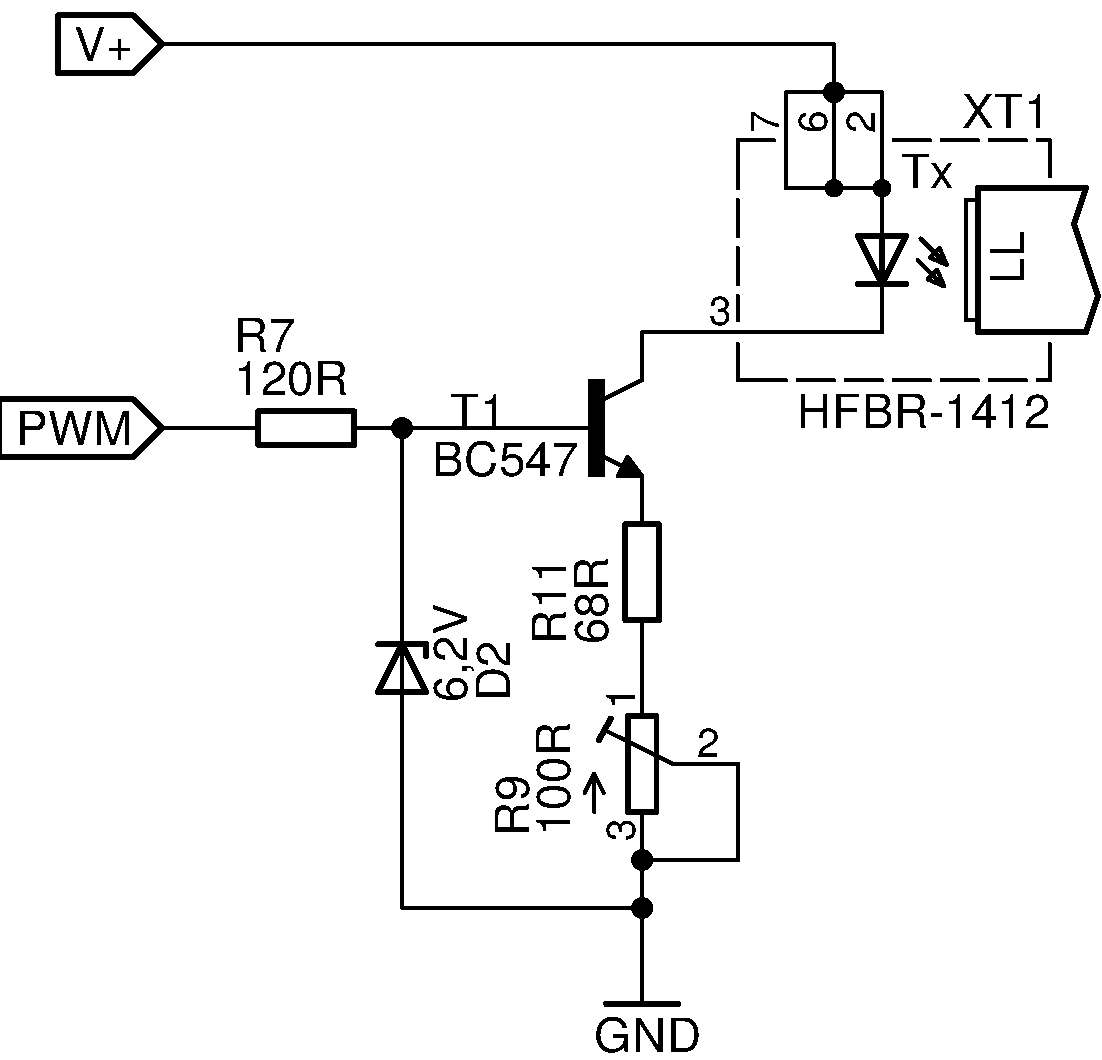
\includegraphics[width=6cm]{gfx/diodentreiber.pdf}
\caption{Diodentreiber}
\label{fig:diodedriver}
\end{floatingfigure}
Als Sendediode wird die Hoch\-leis\-tungs\-diode \textsc{HFBR-1412} verwendet. Diese benötigt minimal $30mA$ und maximal $120mA$. Da eine Diode ein Halbleiter ist, hat diese iene exponentielle Span\-nungs-Strom Kennlinie. Bei einer Versorgung mit konstanter Spannung kann durch thermische Rückkopplung der Strom, und damit die Verlustleistung, unkontrolliert ansteigen. Dies kann zur Zer\-störung des Bauteils führen. Aufgrund dessen wird der Diodentreiber als Kon\-stant\-strom\-quel\-le (KSQ) ausgeführt.

Die KSQ besteht aus $T_1$, $R_{11}$, $R_9$ und $D_2$. Der Widerstand $R_7$ dient lediglich der Begrenzung des Basisstromes von $T_1$ und der Strombegrenzung von $D_2$.
Die Zener-Diode $D_2$ hält die Spannung über der BE-Strecke von $T_1$ und den Widerständen $R_{11}$ und $R_9$ konstant. Da die Spannng über den Widerständen konstant ist, ist auch der Strom durch diese konstant. Daraus folgt, dass auch der Kollektorstrom von $T_1$ und somit auch der Strom durch die Leistungsdiode konstant ist.
Der Strom berechnet sich wie folgt.
\begin{align}
I_{konst} = \frac{U_z-U_{BE}}{R_9+R_{11}}
\end{align} 
Durch den Reihenwiderstand $R_{11}$	ist sichergestellt, dass auch bei Anschlag der Potentiometers zu $0\Omega$ der Strom nicht $130mA$ übersteigt. Der gesamte Einstellbereich für den Diodenstrom liegt bei $36mA < I_{konst}< 110mA$.
\newpage